%-------------------------------------------------------------------------------
\section{Evaluation}
%-------------------------------------------------------------------------------


\subsection{Experimental Setup}
\label{sec:expsetup}

\DZ{Cut some text in this subsection if there is no space}
\DZ{Add citations to the model and workloads.}

\PN{Model and System Configuration.} 
The experiments are conducted on a system equipped with 4 NVIDIA A10 GPUs, each with 24GB of GPU memory.
We employ four representative models in our study: OPT-6.7B and OPT-13B, which are conventional transformer models using Multi-Head Attention~(MHA), 
and Qwen2-7B and Yi-1.5-9B, both of which adopt Grouped-Query Attention (GQA) mechanisms.
Due to the current implementation limitations of \flexgen, which only supports OPT models, 
some experiments involving \flexgen are conducted exclusively on the two OPT models.
%
Unless otherwise specified, all experiments are conducted using chunked prefill and float16 data format.

\PN{Workload.} 
%
\Maphsge{list a table here, like sarathi-serve}
We evaluate our system using two representative workloads. 
LongBench includes tasks with input lengths ranging from 8,000 to 2 million characters, covering diverse long-context scenarios. 
Alpaca is derived from instruction-following outputs of OpenAI's text-davinci-003 engine. 
The requests are submitted at a rate following a Poisson distribution to mimic realistic serving conditions. 

\PN{Baseline.} 
We consider three baselines in our evaluation: DeepSpeed, FlexGen, and a naive method.
The naive method involves loading the entire model into GPU memory without any offloading using vLLM. 

\PN{Key Metrics.} 
%
We use several key metrics to evaluate including host memory usage for memory efficiency, 
\DZ{Add a reference to the subsection where we introduce these two metrics} 
%
TPOT for latency, and throughput for overall inference performance, which measures the number of tokens generated per second.
In order to ensure experimental consistency, the TPOT SLO is set to 100 ms which is higher than the normal human read
speed.

Another critical metric is the maximum allocatable length (\textit{max length}). 
This metric is computed as 
\[
\textit{max length} = \textit{batch size} \times (\textit{sequence length} + \textit{output length}),
\]
where the term captures the total number of tokens that the system can handle for a single model instance. 
A higher \textit{max length} indicates the system's ability to support larger batch sizes, longer input sequences, and extended output sequences.

\begin{figure*}[t]
    \centering
    \resizebox{\textwidth}{!}{
        % This file was created with tikzplotlib v0.10.1.
\begin{tikzpicture}

\definecolor{darkgray176}{RGB}{176,176,176}
\definecolor{green}{RGB}{0,128,0}
\definecolor{lightgray204}{RGB}{204,204,204}
\definecolor{orange}{RGB}{255,165,0}

\begin{groupplot}[group style={group size=6 by 1}]
\nextgroupplot[
legend cell align={left},
legend style={fill opacity=0.8, draw opacity=1, text opacity=1, draw=lightgray204},
tick align=outside,
tick pos=left,
title={(a) OPT Model on Alpaca},
x grid style={darkgray176},
xlabel={Batch Size},
xmin=-0.3, xmax=6.3,
xtick style={color=black},
xtick={0,1,2,3,4,5,6},
xtick={0,1,2,3,4,5,6},
xtick={0,1,2,3,4,5,6},
xtick={0,1,2,3,4,5,6},
xticklabels={2,4,8,16,32,64,128},
xticklabels={2,4,8,16,32,64,128},
xticklabels={2,4,8,16,32,64,128},
xticklabels={2,4,8,16,32,64,128},
y grid style={darkgray176},
ylabel={Latency (ms)},
ymin=-25.51, ymax=535.71,
ytick style={color=black}
]
\addplot [thick, green, mark=*, mark size=3, mark options={solid}]
table {%
0 89.41
1 89.94
2 90.66
3 46.05
4 23.74
5 0
6 0
};
\addlegendentry{\sys-TPOT}
\addplot [very thick, blue, dotted, mark=x, mark size=3, mark options={solid}]
table {%
0 357.6
1 179.9
2 90.66
3 46.05
4 23.74
5 0
6 0
};
\addlegendentry{DeepSpeed-TPOT}
\addplot [very thick, orange, dotted, mark=square*, mark size=3, mark options={solid}]
table {%
0 510.2
1 279.3
2 162.8
3 104.16
4 74.24
5 58.68
6 51.54
};
\addlegendentry{FlexGen-TPOT}

\nextgroupplot[
tick align=outside,
tick pos=left,
title={(b) Qwen2 Model on Alpaca},
x grid style={darkgray176},
xlabel={Batch Size},
xmin=-0.3, xmax=6.3,
xtick style={color=black},
xtick={0,1,2,3,4,5,6},
xtick={0,1,2,3,4,5,6},
xtick={0,1,2,3,4,5,6},
xticklabels={2,4,8,16,32,64,128},
xticklabels={2,4,8,16,32,64,128},
xticklabels={2,4,8,16,32,64,128},
y grid style={darkgray176},
ymin=-0.0855000000000032, ymax=646.1755,
ytick style={color=black}
]
\addplot [thick, green, mark=*, mark size=3, mark options={solid}]
table {%
0 154.2
1 99.13
2 98.89
3 95.18
4 59.27
5 39.31
6 29.29
};
\addplot [very thick, blue, dotted, mark=x, mark size=3, mark options={solid}]
table {%
0 616.8
1 326.13
2 173.81
3 99.007
4 59.27
5 39.41
6 29.29
};

\nextgroupplot[
tick align=outside,
tick pos=left,
title={(c) Qwen Model on Alpaca},
x grid style={darkgray176},
xlabel={Batch Size},
xmin=-0.3, xmax=6.3,
xtick style={color=black},
xtick={0,1,2,3,4,5,6},
xtick={0,1,2,3,4,5,6},
xtick={0,1,2,3,4,5,6},
xticklabels={2,4,8,16,32,64,128},
xticklabels={2,4,8,16,32,64,128},
xticklabels={2,4,8,16,32,64,128},
y grid style={darkgray176},
ymin=-4.4751, ymax=792.2131,
ytick style={color=black}
]
\addplot [thick, green, mark=*, mark size=3, mark options={solid}]
table {%
0 390
1 195
2 97.65
3 95.18
4 61.48
5 43.68
6 31.738
};
\addplot [very thick, blue, dotted, mark=x, mark size=3, mark options={solid}]
table {%
0 756
1 382
2 195
3 105.27
4 61.48
5 43.68
6 31.738
};

\nextgroupplot[
tick align=outside,
tick pos=left,
title={(d) OPT Model on LongBench},
x grid style={darkgray176},
xlabel={Batch Size},
xmin=-0.3, xmax=6.3,
xtick style={color=black},
xtick={0,1,2,3,4,5,6},
xtick={0,1,2,3,4,5,6},
xtick={0,1,2,3,4,5,6},
xtick={0,1,2,3,4,5,6},
xticklabels={2,4,8,16,32,64,128},
xticklabels={2,4,8,16,32,64,128},
xticklabels={2,4,8,16,32,64,128},
xticklabels={2,4,8,16,32,64,128},
y grid style={darkgray176},
ymin=-53.15, ymax=1116.15,
ytick style={color=black}
]
\addplot [thick, green, mark=*, mark size=3, mark options={solid}]
table {%
0 0
1 89.87
2 90.47
3 45.83
4 23.51
5 0
6 0
};
\addplot [very thick, blue, dotted, mark=x, mark size=3, mark options={solid}]
table {%
0 0
1 180
2 90.47
3 45.83
4 23.51
5 0
6 0
};
\addplot [very thick, orange, dotted, mark=square*, mark size=3, mark options={solid}]
table {%
0 1063
1 826
2 502
3 429
4 390
5 364
6 340
};

\nextgroupplot[
tick align=outside,
tick pos=left,
title={(e) Qwen2 Model on LongBench},
x grid style={darkgray176},
xlabel={Batch Size},
xmin=-0.3, xmax=6.3,
xtick style={color=black},
xtick={0,1,2,3,4,5,6},
xtick={0,1,2,3,4,5,6},
xtick={0,1,2,3,4,5,6},
xticklabels={2,4,8,16,32,64,128},
xticklabels={2,4,8,16,32,64,128},
xticklabels={2,4,8,16,32,64,128},
y grid style={darkgray176},
ymin=-52.023, ymax=1092.483,
ytick style={color=black}
]
\addplot [thick, green, mark=*, mark size=3, mark options={solid}]
table {%
0 0
1 260.114
2 149.6
3 94.74
4 97.21875
5 0
6 0
};
\addplot [very thick, blue, dotted, mark=x, mark size=3, mark options={solid}]
table {%
0 0
1 1040.46
2 523.68
3 265.3
4 136.1
5 0
6 0
};

\nextgroupplot[
tick align=outside,
tick pos=left,
title={(f) Yi Model on LongBench},
x grid style={darkgray176},
xlabel={Batch Size},
xmin=-0.3, xmax=6.3,
xtick style={color=black},
xtick={0,1,2,3,4,5,6},
xtick={0,1,2,3,4,5,6},
xtick={0,1,2,3,4,5,6},
xticklabels={2,4,8,16,32,64,128},
xticklabels={2,4,8,16,32,64,128},
xticklabels={2,4,8,16,32,64,128},
y grid style={darkgray176},
ymin=-52.0574, ymax=1093.2054,
ytick style={color=black}
]
\addplot [thick, green, mark=*, mark size=3, mark options={solid}]
table {%
0 0
1 260.2
2 131.1805
3 95.18
4 98.25
5 0
6 0
};
\addplot [very thick, blue, dotted, mark=x, mark size=3, mark options={solid}]
table {%
0 0
1 1041.148
2 524.722
3 266.509
4 137.4
5 0
6 0
};
\end{groupplot}

\end{tikzpicture}
 % 插入 TikZ 图
 }
    \caption{Comparison of TPOT under different models and workloads. }
    \label{fig:eval1}
\end{figure*}

\subsection{Maintaining SLO}

We first evaluate \sys's ability to maintain SLO with different batch sizes. 
The results presented in Figure~\ref{fig:eval1} clearly demonstrate that \sys effectively maintains the specified SLO across different setups. 
This is because \sys adjusts the \interval parameter according to the batch size to maintain the SLOs. 
%

In comparison, DeepSpeed fails to meet the specified SLOs, \Maphsge{Add \flexgen and naive}
with TPOT latencies exceeding the target by a factor of 8.08x. This is because \deepspeed always keeps the minimal portion fixed on the GPU.
\Maphsge{this reason is the same as the one in the throughput section.}


\subsection{Throughput Comparison}
\label{sec:memsave}

We conduct experiments to evaluate and compare \sys and other baselines in terms of throughput performance under various models and input conditions. 
Figure~\ref{fig:eval2}(a) presents the results of the throughput comparison. 

\sys outperforms \deepspeed in throughput by a factor of 6.8× to 8.23×. 
This is because, as shown in the Figure~\ref{fig:eval2}(b), under the chunked prefill mode \Maphsge{fig here is chunked under different batch sizes}, 
the transfer time of a single decoder layer significantly exceeds its computation time. 
Since \deepspeed incur transfer overhead at every layer, it requires substantially more time to generate the same number of tokens.

\sys consistently achieves higher throughput than \flexgen and achieves up to 1.85\X the throughput of \flexgen in the best case. 
This is because \flexgen's memory-saving capability is consistently inferior to that of \sys at the same batch size 
due to inaccuracies in its estimation of transfer and computation latencies, 
resulting in suboptimal offloading decisions. As shown in the Figure~\ref{fig:eval2}(c), \sys achieves 2.37\X better memory savings compared to \flexgen. 
By saving more memory, \sys can support larger input scales, which further enhances throughput. 
This advantage will be discussed in greater detail in Section~\S\ref{sec:benefits}.

\begin{figure}[t]
    \centering
    \resizebox{\columnwidth}{!}{
        % This file was created with tikzplotlib v0.10.1.
\begin{tikzpicture}

\definecolor{chocolate213940}{RGB}{213,94,0}
\definecolor{cornflowerblue93173226}{RGB}{93,173,226}
\definecolor{darkgray176}{RGB}{176,176,176}
\definecolor{gold}{RGB}{255,215,0}
\definecolor{mediumvioletred16632106}{RGB}{166,32,106}

\begin{groupplot}[group style={group size=2 by 2}]
\nextgroupplot[
legend cell align={left},
legend style={
  fill opacity=0.8,
  draw opacity=1,
  text opacity=1,
  at={(0.03,0.97)},
  anchor=north west,
  draw=none
},
tick align=outside,
tick pos=left,
title={(a) Memory Usage on Alpaca},
x grid style={darkgray176},
xlabel={Batch Size},
xmin=-0.535, xmax=3.535,
xtick style={color=black},
xtick={0,1,2,3},
xticklabels={8,32,64,128},
y grid style={darkgray176},
ylabel={Memory Usage (GB)},
ymin=0, ymax=12.5685,
ytick style={color=black}
]
\draw[draw=none,fill=cornflowerblue93173226] (axis cs:-0.35,0) rectangle (axis cs:0,7.77);
\addlegendimage{ybar,ybar legend,draw=none,fill=cornflowerblue93173226}
\addlegendentry{NovaServe}

\draw[draw=none,fill=cornflowerblue93173226] (axis cs:0.65,0) rectangle (axis cs:1,7.77);
\draw[draw=none,fill=cornflowerblue93173226] (axis cs:1.65,0) rectangle (axis cs:2,11.97);
\draw[draw=none,fill=cornflowerblue93173226] (axis cs:2.65,0) rectangle (axis cs:3,11.97);
\draw[draw=gold,fill=white,postaction={pattern=north east lines, pattern color=gold}] (axis cs:2.77555756156289e-17,0) rectangle (axis cs:0.35,4.672);
\addlegendimage{ybar,ybar legend,draw=gold,fill=white,postaction={pattern=north east lines, pattern color=gold}}
\addlegendentry{FlexGen}

\draw[draw=gold,fill=white,postaction={pattern=north east lines, pattern color=gold}] (axis cs:1,0) rectangle (axis cs:1.35,4.8);
\draw[draw=gold,fill=white,postaction={pattern=north east lines, pattern color=gold}] (axis cs:2,0) rectangle (axis cs:2.35,5.05);
\draw[draw=gold,fill=white,postaction={pattern=north east lines, pattern color=gold}] (axis cs:3,0) rectangle (axis cs:3.35,5.57);
\draw (axis cs:-0.2,7.97) node[
  scale=0.5,
  anchor=base,
  text=black,
  rotate=0.0
]{7.77};
\draw (axis cs:0.8,7.97) node[
  scale=0.5,
  anchor=base,
  text=black,
  rotate=0.0
]{7.77};
\draw (axis cs:1.8,12.17) node[
  scale=0.5,
  anchor=base,
  text=black,
  rotate=0.0
]{11.97};
\draw (axis cs:2.8,12.17) node[
  scale=0.5,
  anchor=base,
  text=black,
  rotate=0.0
]{11.97};
\draw (axis cs:0.2,4.872) node[
  scale=0.5,
  anchor=base,
  text=black,
  rotate=0.0
]{4.67};
\draw (axis cs:1.2,5) node[
  scale=0.5,
  anchor=base,
  text=black,
  rotate=0.0
]{4.80};
\draw (axis cs:2.2,5.25) node[
  scale=0.5,
  anchor=base,
  text=black,
  rotate=0.0
]{5.05};
\draw (axis cs:3.2,5.77) node[
  scale=0.5,
  anchor=base,
  text=black,
  rotate=0.0
]{5.57};

\nextgroupplot[
legend cell align={left},
legend style={
  fill opacity=0.8,
  draw opacity=1,
  text opacity=1,
  at={(0.03,0.97)},
  anchor=north west,
  draw=none
},
tick align=outside,
tick pos=left,
title={(b) Memory Usage on LongBench},
x grid style={darkgray176},
xlabel={Batch Size},
xmin=-0.535, xmax=3.535,
xtick style={color=black},
xtick={0,1,2,3},
xticklabels={8,32,64,128},
y grid style={darkgray176},
ymin=0, ymax=12.5685,
ytick style={color=black}
]
\draw[draw=none,fill=cornflowerblue93173226] (axis cs:-0.35,0) rectangle (axis cs:0,7.77);
\draw[draw=none,fill=cornflowerblue93173226] (axis cs:0.65,0) rectangle (axis cs:1,7.77);
\draw[draw=none,fill=cornflowerblue93173226] (axis cs:1.65,0) rectangle (axis cs:2,11.97);
\draw[draw=none,fill=cornflowerblue93173226] (axis cs:2.65,0) rectangle (axis cs:3,11.97);
\draw[draw=gold,fill=white,postaction={pattern=north east lines, pattern color=gold}] (axis cs:2.77555756156289e-17,0) rectangle (axis cs:0.35,4.672);
\draw[draw=gold,fill=white,postaction={pattern=north east lines, pattern color=gold}] (axis cs:1,0) rectangle (axis cs:1.35,4.8);
\draw[draw=gold,fill=white,postaction={pattern=north east lines, pattern color=gold}] (axis cs:2,0) rectangle (axis cs:2.35,5.05);
\draw[draw=gold,fill=white,postaction={pattern=north east lines, pattern color=gold}] (axis cs:3,0) rectangle (axis cs:3.35,5.57);
\draw (axis cs:-0.2,7.97) node[
  scale=0.5,
  anchor=base,
  text=black,
  rotate=0.0
]{7.77};
\draw (axis cs:0.8,7.97) node[
  scale=0.5,
  anchor=base,
  text=black,
  rotate=0.0
]{7.77};
\draw (axis cs:1.8,12.17) node[
  scale=0.5,
  anchor=base,
  text=black,
  rotate=0.0
]{11.97};
\draw (axis cs:2.8,12.17) node[
  scale=0.5,
  anchor=base,
  text=black,
  rotate=0.0
]{11.97};
\draw (axis cs:0.2,4.872) node[
  scale=0.5,
  anchor=base,
  text=black,
  rotate=0.0
]{4.67};
\draw (axis cs:1.2,5) node[
  scale=0.5,
  anchor=base,
  text=black,
  rotate=0.0
]{4.80};
\draw (axis cs:2.2,5.25) node[
  scale=0.5,
  anchor=base,
  text=black,
  rotate=0.0
]{5.05};
\draw (axis cs:3.2,5.77) node[
  scale=0.5,
  anchor=base,
  text=black,
  rotate=0.0
]{5.57};

\nextgroupplot[
legend cell align={left},
legend style={
  fill opacity=0.8,
  draw opacity=1,
  text opacity=1,
  at={(0.03,0.97)},
  anchor=north west,
  draw=none
},
tick align=outside,
tick pos=left,
title={(c) Throughput Comparison on Alpaca},
x grid style={darkgray176},
xlabel={Batch Size},
xmin=-0.535, xmax=3.535,
xtick style={color=black},
xtick={0,1,2,3},
xticklabels={8,32,64,128},
y grid style={darkgray176},
ylabel={Throughput (tokens/s)},
ymin=0, ymax=59.997,
ytick style={color=black}
]
\draw[draw=none,fill=chocolate213940] (axis cs:-0.35,0) rectangle (axis cs:0,10.25);
\draw[draw=none,fill=chocolate213940] (axis cs:0.65,0) rectangle (axis cs:1,21.97);
\draw[draw=none,fill=chocolate213940] (axis cs:1.65,0) rectangle (axis cs:2,28.57);
\draw[draw=none,fill=chocolate213940] (axis cs:2.65,0) rectangle (axis cs:3,57.14);
\draw[draw=mediumvioletred16632106,fill=white,postaction={pattern=north east lines, pattern color=mediumvioletred16632106}] (axis cs:2.77555756156289e-17,0) rectangle (axis cs:0.35,8.94);
\draw[draw=mediumvioletred16632106,fill=white,postaction={pattern=north east lines, pattern color=mediumvioletred16632106}] (axis cs:1,0) rectangle (axis cs:1.35,11.85);
\draw[draw=mediumvioletred16632106,fill=white,postaction={pattern=north east lines, pattern color=mediumvioletred16632106}] (axis cs:2,0) rectangle (axis cs:2.35,25.5);
\draw[draw=mediumvioletred16632106,fill=white,postaction={pattern=north east lines, pattern color=mediumvioletred16632106}] (axis cs:3,0) rectangle (axis cs:3.35,35.46);
\draw (axis cs:-0.2,12.25) node[
  scale=0.5,
  anchor=base,
  text=black,
  rotate=0.0
]{10.25};
\draw (axis cs:0.8,23.97) node[
  scale=0.5,
  anchor=base,
  text=black,
  rotate=0.0
]{21.97};
\draw (axis cs:1.8,30.57) node[
  scale=0.5,
  anchor=base,
  text=black,
  rotate=0.0
]{28.57};
\draw (axis cs:2.8,59.14) node[
  scale=0.5,
  anchor=base,
  text=black,
  rotate=0.0
]{57.14};
\draw (axis cs:0.2,10.94) node[
  scale=0.5,
  anchor=base,
  text=black,
  rotate=0.0
]{8.94};
\draw (axis cs:1.2,13.85) node[
  scale=0.5,
  anchor=base,
  text=black,
  rotate=0.0
]{11.85};
\draw (axis cs:2.2,27.5) node[
  scale=0.5,
  anchor=base,
  text=black,
  rotate=0.0
]{25.50};
\draw (axis cs:3.2,37.46) node[
  scale=0.5,
  anchor=base,
  text=black,
  rotate=0.0
]{35.46};

\nextgroupplot[
legend cell align={left},
legend style={
  fill opacity=0.8,
  draw opacity=1,
  text opacity=1,
  at={(0.03,0.97)},
  anchor=north west,
  draw=none
},
tick align=outside,
tick pos=left,
title={(d) Throughput Comparison on LongBench},
x grid style={darkgray176},
xlabel={Batch Size},
xmin=-0.535, xmax=3.535,
xtick style={color=black},
xtick={0,1,2,3},
xticklabels={8,32,64,128},
y grid style={darkgray176},
ymin=0, ymax=59.997,
ytick style={color=black}
]
\draw[draw=none,fill=chocolate213940] (axis cs:-0.35,0) rectangle (axis cs:0,10.25);
\draw[draw=none,fill=chocolate213940] (axis cs:0.65,0) rectangle (axis cs:1,21.97);
\draw[draw=none,fill=chocolate213940] (axis cs:1.65,0) rectangle (axis cs:2,28.57);
\draw[draw=none,fill=chocolate213940] (axis cs:2.65,0) rectangle (axis cs:3,57.14);
\draw[draw=mediumvioletred16632106,fill=white,postaction={pattern=north east lines, pattern color=mediumvioletred16632106}] (axis cs:2.77555756156289e-17,0) rectangle (axis cs:0.35,8.94);
\draw[draw=mediumvioletred16632106,fill=white,postaction={pattern=north east lines, pattern color=mediumvioletred16632106}] (axis cs:1,0) rectangle (axis cs:1.35,11.85);
\draw[draw=mediumvioletred16632106,fill=white,postaction={pattern=north east lines, pattern color=mediumvioletred16632106}] (axis cs:2,0) rectangle (axis cs:2.35,25.5);
\draw[draw=mediumvioletred16632106,fill=white,postaction={pattern=north east lines, pattern color=mediumvioletred16632106}] (axis cs:3,0) rectangle (axis cs:3.35,35.46);
\draw (axis cs:-0.2,12.25) node[
  scale=0.5,
  anchor=base,
  text=black,
  rotate=0.0
]{10.25};
\draw (axis cs:0.8,23.97) node[
  scale=0.5,
  anchor=base,
  text=black,
  rotate=0.0
]{21.97};
\draw (axis cs:1.8,30.57) node[
  scale=0.5,
  anchor=base,
  text=black,
  rotate=0.0
]{28.57};
\draw (axis cs:2.8,59.14) node[
  scale=0.5,
  anchor=base,
  text=black,
  rotate=0.0
]{57.14};
\draw (axis cs:0.2,10.94) node[
  scale=0.5,
  anchor=base,
  text=black,
  rotate=0.0
]{8.94};
\draw (axis cs:1.2,13.85) node[
  scale=0.5,
  anchor=base,
  text=black,
  rotate=0.0
]{11.85};
\draw (axis cs:2.2,27.5) node[
  scale=0.5,
  anchor=base,
  text=black,
  rotate=0.0
]{25.50};
\draw (axis cs:3.2,37.46) node[
  scale=0.5,
  anchor=base,
  text=black,
  rotate=0.0
]{35.46};
\end{groupplot}

\end{tikzpicture}
 % 插入 TikZ 图
 }
    \caption{(a) (b) Memory usage on the offloading devices for \sys and FlexGen under different batch sizes. 
 (c) (d) Throughput comparison between \sys and FlexGen under different batch sizes.}
    \label{fig:eval2}
\end{figure}

\subsection{Benefits of \sys}
\label{sec:benefits}

\PN{Supporting larger models.}
\Maphsge{I wonder if we still need this section because all the experiments above is based on this.}
\sys is capable of supporting models whose memory demands exceed the GPU memory capacity, as demonstrated in experiments with OPT-13B (using float16 data format), 
Qwen2-7B, and GLM-4-9B (both using float32 data format).
Figure~\ref{fig:eval3} presents the TPOT performance of different models respectively, under varying batch sizes. All models, 
which require memory beyond the 24GB GPU capacity in our setup, were successfully executed using \sys. 
TPOT values below 100 ms are higher than the normal human reading speed, indicating that such latencies allow for efficient and real-time text generation. 
In our experiments, the TPOT values for the three models remained consistently below 100ms across most tested batch sizes except for scenarios where the batch size 
is set too small, demonstrating that \sys satisfies the SLO in most cases.
This confirms that \sys not only enables the execution of these large-scale models but also ensures efficient performance suitable for real-world applications.

\begin{figure}[t]
    \centering
    \resizebox{0.5\columnwidth}{!}{
        % This file was created with tikzplotlib v0.10.1.
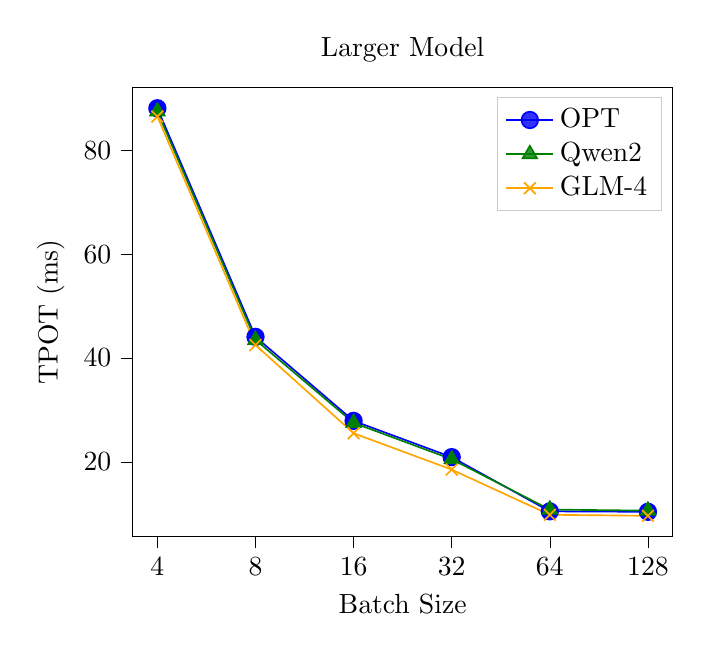
\begin{tikzpicture}

\definecolor{darkgray176}{RGB}{176,176,176}
\definecolor{green}{RGB}{0,128,0}
\definecolor{lightgray204}{RGB}{204,204,204}
\definecolor{orange}{RGB}{255,165,0}

\begin{axis}[
legend cell align={left},
legend style={fill opacity=0.8, draw opacity=1, text opacity=1, draw=lightgray204},
tick align=outside,
tick pos=left,
title={Larger Model},
x grid style={darkgray176},
xlabel={Batch Size},
xmin=-0.25, xmax=5.25,
xtick style={color=black},
xtick={0,1,2,3,4,5},
xtick={0,1,2,3,4,5},
xtick={0,1,2,3,4,5},
xtick={0,1,2,3,4,5},
xticklabels={4,8,16,32,64,128},
xticklabels={4,8,16,32,64,128},
xticklabels={4,8,16,32,64,128},
xticklabels={4,8,16,32,64,128},
y grid style={darkgray176},
ylabel={TPOT (ms)},
ymin=5.675, ymax=92.025,
ytick style={color=black}
]
\addplot [semithick, blue, mark=*, mark size=3, mark options={solid}]
table {%
0 88.1
1 44.066
2 27.8875
3 20.9
4 10.46
5 10.37
};
\addlegendentry{OPT}
\addplot [semithick, green, mark=triangle*, mark size=3, mark options={solid}]
table {%
0 87.5
1 43.5
2 27.5
3 20.5
4 10.8
5 10.6
};
\addlegendentry{Qwen2}
\addplot [semithick, orange, mark=x, mark size=3, mark options={solid}]
table {%
0 86.5
1 42.5
2 25.5
3 18.5
4 9.8
5 9.6
};
\addlegendentry{GLM-4}
\end{axis}

\end{tikzpicture}
 % 插入 TikZ 图
 }
    \caption{TPOT of different models using \sys.}
    \label{fig:eval3}
\end{figure}

\PN{Supporting more input and output tokens.}
In our experiments, we use the Qwen2-7B model, which support a maximum position embedding size of 32,768 tokens. 
This choice is deliberate, 
as this model significantly exceed the position embedding limits of OPT models and Yi-1.5 model, 
ensuring that the system remains capable of processing long input sequences. 
To compare with \flexgen, we calculate the corresponding offloading ratio based on the \interval values used in \sys and then manually set this ratio in \flexgen. 
We also conducted comparisons with \deepspeed.

The results in Figure~\ref{fig:eval4} show that, 
\sys supports larger max length than others. 
This is because reducing the GPU memory using allows \sys to allocate more GPU memory for token processing, thereby increasing the maximum allocatable length. 
As a result, the system can support larger batch sizes, 
longer input sequences, or extended output sequences under different interval settings, which helps to improve throughput. 
In contrast, \flexgen consistently shows smaller max length than \sys, while \deepspeed always retains one layer in GPU HBM, 
resulting in a constant larger value in the graph.

\begin{figure}[t]
    \centering
    \resizebox{\columnwidth}{!}{
        % This file was created with tikzplotlib v0.10.1.
\begin{tikzpicture}

\definecolor{darkgray176}{RGB}{176,176,176}
\definecolor{darkorange25512714}{RGB}{255,127,14}
\definecolor{forestgreen4416044}{RGB}{44,160,44}
\definecolor{lightgray204}{RGB}{204,204,204}
\definecolor{steelblue31119180}{RGB}{31,119,180}

\begin{groupplot}[group style={group size=2 by 1}]
\nextgroupplot[
legend cell align={left},
legend style={
  fill opacity=0.8,
  draw opacity=1,
  text opacity=1,
  at={(0.91,0.5)},
  anchor=east,
  draw=lightgray204
},
tick align=outside,
tick pos=left,
title={Qwen2 Model},
x grid style={darkgray176},
xlabel={Interval},
xmajorgrids,
xmin=1.7, xmax=8.3,
xtick style={color=black},
y grid style={darkgray176},
ylabel={Max Length},
ymajorgrids,
ymin=7835.44, ymax=25817.36,
ytick style={color=black}
]
\addplot [semithick, steelblue31119180, mark=*, mark size=3, mark options={solid}]
table {%
2 20080
3 15440
4 13904
5 12352
6 11584
7 10816
8 10816
};
\addlegendentry{Original}
\addplot [semithick, darkorange25512714, mark=triangle*, mark size=3, mark options={solid}]
table {%
2 16064
3 12352
4 11123.2
5 9881.6
6 9267.2
7 8652.8
8 8652.8
};
\addlegendentry{FlexGen}
\addplot [semithick, forestgreen4416044, dashed]
table {%
1.7 25000
8.3 25000
};
\addlegendentry{DeepSpeed}
\addplot [semithick, red, dashed]
table {%
1.7 9376
8.3 9376
};
\addlegendentry{Naive}

\nextgroupplot[
legend cell align={left},
legend style={
  fill opacity=0.8,
  draw opacity=1,
  text opacity=1,
  at={(0.91,0.5)},
  anchor=east,
  draw=lightgray204
},
tick align=outside,
tick pos=left,
title={GLM-4 Model},
x grid style={darkgray176},
xlabel={Interval},
xmajorgrids,
xmin=1.7, xmax=8.3,
xtick style={color=black},
y grid style={darkgray176},
ylabel={Max Length},
ymajorgrids,
ymin=7835.44, ymax=25817.36,
ytick style={color=black}
]
\addplot [semithick, steelblue31119180, mark=*, mark size=3, mark options={solid}]
table {%
2 20080
3 15440
4 13904
5 12352
6 11584
7 10816
8 10816
};
\addlegendentry{Original}
\addplot [semithick, darkorange25512714, mark=triangle*, mark size=3, mark options={solid}]
table {%
2 16064
3 12352
4 11123.2
5 9881.6
6 9267.2
7 8652.8
8 8652.8
};
\addlegendentry{FlexGen}
\addplot [semithick, forestgreen4416044, dashed]
table {%
1.7 25000
8.3 25000
};
\addlegendentry{DeepSpeed}
\addplot [semithick, red, dashed]
table {%
1.7 9376
8.3 9376
};
\addlegendentry{Naive}
\end{groupplot}

\end{tikzpicture}
 % 插入 TikZ 图
 }
    \caption{Maximum prompt length the model can process under different \interval settings.
 The dashed line represents the maximum length in the naive mode.}
    \label{fig:eval4}
\end{figure}



\subsection{Profiling Accuracy}

This subsection evaluates the effectiveness of the \interval analyzer, namely examining the optimality of the \interval value determined during the record-generating phase. 
\Maphsge{batch size to 128. }
Based on the optimal \interval value from the records, we conducted experiments under both the optimal and alternative \interval configurations, 
evaluating TPOT latency and recording the corresponding GPU memory usage for each setting.

The results are shown in Figure~\ref{fig:profileraccu}. 
According to performance records, the optimal \interval values are identified as 3 for the Qwen2 and GLM-4 models and 4 for the OPT and LLaMA model. 
The optimal \interval values achieve an effective balance by ensuring compliance with TPOT SLO while minimizing GPU memory usage. 
When \interval is smaller than the optimal value, GPU memory usage is reduced; 
however, this comes at the cost of SLO violations due to increased latency resulting in degraded throughput. 

\Maphsge{shown in fig, larger...}
In contrast, larger \interval values consistently satisfy the SLO but incur significant memory overhead without measurable performance gains. 
Specially, when the model size exceeds the available GPU memory, there is a practical upper bound on the \interval setting. 
As illustrated in the results for the OPT-13B model, which has a size of 26GB, this exceeds the 24GB GPU memory of the A10 GPU. 
Consequently, when the \interval value surpasses 5, the model cannot be deployed due to out-of-memory (OOM) errors.

\begin{figure}[t]
    \centering
    \resizebox{\columnwidth}{!}{
        % This file was created with tikzplotlib v0.10.1.
\begin{tikzpicture}

\definecolor{crimson2143940}{RGB}{214,39,40}
\definecolor{darkgray176}{RGB}{176,176,176}
\definecolor{forestgreen4416044}{RGB}{44,160,44}
\definecolor{lightgray204}{RGB}{204,204,204}
\definecolor{steelblue31119180}{RGB}{31,119,180}

\begin{groupplot}[group style={group size=2 by 1}]
\nextgroupplot[
legend cell align={left},
legend style={fill opacity=0.8, draw opacity=1, text opacity=1, draw=lightgray204},
tick align=outside,
tick pos=left,
title={(a) TPOT Analysis},
x grid style={darkgray176},
xlabel={Interval Configuration},
xmin=-0.56125, xmax=4.08625,
xtick style={color=black},
xtick={0,1.175,2.35,3.525},
xticklabels={5,6,8,10},
y grid style={darkgray176},
ylabel={TPOT},
ymin=0, ymax=130.1265,
ytick style={color=black}
]
\draw[draw=none,fill=steelblue31119180] (axis cs:-0.35,0) rectangle (axis cs:0,123.93);
\addlegendimage{ybar,ybar legend,draw=none,fill=steelblue31119180}
\addlegendentry{OPT}

\draw[draw=none,fill=steelblue31119180] (axis cs:0.825,0) rectangle (axis cs:1.175,115.03);
\draw[draw=none,fill=steelblue31119180] (axis cs:2,0) rectangle (axis cs:2.35,89.388);
\draw[draw=none,fill=steelblue31119180] (axis cs:3.175,0) rectangle (axis cs:3.525,68.17);
\draw[draw=forestgreen4416044,fill=white,postaction={pattern=north east lines, pattern color=forestgreen4416044}] (axis cs:2.77555756156289e-17,0) rectangle (axis cs:0.35,123.93);
\addlegendimage{ybar,ybar legend,draw=forestgreen4416044,fill=white,postaction={pattern=north east lines, pattern color=forestgreen4416044}}
\addlegendentry{Qwen2}

\draw[draw=forestgreen4416044,fill=white,postaction={pattern=north east lines, pattern color=forestgreen4416044}] (axis cs:1.175,0) rectangle (axis cs:1.525,115.03);
\draw[draw=forestgreen4416044,fill=white,postaction={pattern=north east lines, pattern color=forestgreen4416044}] (axis cs:2.35,0) rectangle (axis cs:2.7,89.388);
\draw[draw=forestgreen4416044,fill=white,postaction={pattern=north east lines, pattern color=forestgreen4416044}] (axis cs:3.525,0) rectangle (axis cs:3.875,68.17);
\addplot [semithick, crimson2143940, dashed]
table {%
-0.56125 90
4.08625 90
};
\addlegendentry{SLO}

\nextgroupplot[
legend cell align={left},
legend style={
  fill opacity=0.8,
  draw opacity=1,
  text opacity=1,
  at={(0.03,0.97)},
  anchor=north west,
  draw=lightgray204
},
tick align=outside,
tick pos=left,
title={(b) Memory Usage Analysis},
x grid style={darkgray176},
xlabel={Configuration},
xmin=-0.7375, xmax=7.7875,
xtick style={color=black},
xtick={0,1.175,2.35,3.525,4.7,5.875,7.05},
xticklabels={2,3,4,5,6,8,10},
y grid style={darkgray176},
ylabel={Memory Usage (GB)},
ymin=0, ymax=22.96875,
ytick style={color=black}
]
\draw[draw=none,fill=steelblue31119180] (axis cs:-0.35,0) rectangle (axis cs:0,11.5);
\draw[draw=none,fill=steelblue31119180] (axis cs:0.825,0) rectangle (axis cs:1.175,15.8);
\draw[draw=none,fill=steelblue31119180] (axis cs:2,0) rectangle (axis cs:2.35,17.25);
\draw[draw=none,fill=steelblue31119180] (axis cs:3.175,0) rectangle (axis cs:3.525,18.69);
\draw[draw=none,fill=steelblue31119180] (axis cs:4.35,0) rectangle (axis cs:4.7,21.125);
\draw[draw=none,fill=steelblue31119180] (axis cs:5.525,0) rectangle (axis cs:5.875,21.5);
\draw[draw=none,fill=steelblue31119180] (axis cs:6.7,0) rectangle (axis cs:7.05,21.875);
\draw[draw=forestgreen4416044,fill=white,postaction={pattern=north east lines, pattern color=forestgreen4416044}] (axis cs:2.77555756156289e-17,0) rectangle (axis cs:0.35,11.5);
\draw[draw=forestgreen4416044,fill=white,postaction={pattern=north east lines, pattern color=forestgreen4416044}] (axis cs:1.175,0) rectangle (axis cs:1.525,15.8);
\draw[draw=forestgreen4416044,fill=white,postaction={pattern=north east lines, pattern color=forestgreen4416044}] (axis cs:2.35,0) rectangle (axis cs:2.7,17.25);
\draw[draw=forestgreen4416044,fill=white,postaction={pattern=north east lines, pattern color=forestgreen4416044}] (axis cs:3.525,0) rectangle (axis cs:3.875,18.69);
\draw[draw=forestgreen4416044,fill=white,postaction={pattern=north east lines, pattern color=forestgreen4416044}] (axis cs:4.7,0) rectangle (axis cs:5.05,21.125);
\draw[draw=forestgreen4416044,fill=white,postaction={pattern=north east lines, pattern color=forestgreen4416044}] (axis cs:5.875,0) rectangle (axis cs:6.225,21.5);
\draw[draw=forestgreen4416044,fill=white,postaction={pattern=north east lines, pattern color=forestgreen4416044}] (axis cs:7.05,0) rectangle (axis cs:7.4,21.875);
\end{groupplot}

\end{tikzpicture}
 % 插入 TikZ 图
 }
    \caption{The TTFT, TPOT, and memory usage of \sys under different \interval configurations. 
 The red dashed lines represent the SLO. The optimal \interval is 3 in (a) and 8 in (b).}
    \label{fig:profileraccu}
\end{figure}

\DZ{Missing breakdown analysis.}
\subsection{Latency Breakdown}
\Maphsge{Add a figure here.}

To understand \sys's performance in detail, we conduct a latency breakdown analysis of its execution process. 
Specifically, we divide the lifecycle of a single iteration in \sys into the following stages: inference execution, transfer blocking, and \interval adjustment. 
For each stage, we accumulate the total time consumed across all requests to determine its proportion in the overall system execution time. 
We compare \sys with other baseline systems, selecting the OPT-13B model for evaluation since it is natively supported by \flexgen. 

The results of the latency breakdown are illustrated in Figure~X. 
As shown, the primary performance bottleneck in \deepspeed lies in data transfer overhead, which accounts for X\% of the total execution time—significantly 
higher than that in \sys. Although \flexgen exhibits slightly lower data transfer overhead compared to \sys, 
this is largely attributed to its insufficient utilization of host memory resources. 
On the other hand, the overhead introduced by \interval adjustment in \sys is minimal, occupying only a negligible portion of the iteration lifecycle. 

\subsection{Bandwidth contention}

We conduct experiments simulating a scenario where two GPUs share PCIe bandwidth. In this setup, we run inference tasks on both GPUs simultaneously, 
measuring SLO and throughput. Specifically, we run the OPT model on FlexGen, while conducting experiments with different models on \sys. 

Figure~\ref{fig:evalband}(a) shows the SLO results, where \sys consistently maintains the SLO, while FlexGen fails to do so. 
This is because FlexGen lacks the ability to dynamically adjust the offload ratio, whereas \sys can adaptively adjust the \interval to reduce data transfers. 
As a result, FlexGen exhibits lower throughput compared to \sys, as shown in Figure~\ref{fig:evalband}(b).


\begin{figure}[t]
    \centering
    \resizebox{0.9\columnwidth}{!}{
        % This file was created with tikzplotlib v0.10.1.
\begin{tikzpicture}

\definecolor{chocolate213940}{RGB}{213,94,0}
\definecolor{darkgray176}{RGB}{176,176,176}
\definecolor{darkgreen}{RGB}{0,100,0}
\definecolor{darkorange}{RGB}{255,140,0}
\definecolor{gray}{RGB}{128,128,128}

\begin{axis}[
height=6cm,
legend cell align={left},
legend columns=3,
legend style={fill opacity=0.8, draw opacity=1, text opacity=1, at={(0.5,1.2)}, anchor=north, draw=none},
tick align=outside,
tick pos=left,
width=14cm,
x grid style={darkgray176},
xlabel={Batch Size},
xmin=-0.662, xmax=4.662,
xtick style={color=black},
xtick={0,1,2,3,4},
xticklabels={4,8,16,32,64},
y grid style={darkgray176},
ylabel={TPOT (ms)},
ymin=0, ymax=166.95,
ytick style={color=black}
]
\draw[draw=none,fill=chocolate213940] (axis cs:-0.42,0) rectangle (axis cs:-0.14,154);
\addlegendimage{ybar,ybar legend,draw=none,fill=chocolate213940}
\addlegendentry{NovaServe-OPT}

\draw[draw=none,fill=chocolate213940] (axis cs:0.58,0) rectangle (axis cs:0.86,76.99);
\draw[draw=none,fill=chocolate213940] (axis cs:1.58,0) rectangle (axis cs:1.86,39.91);
\draw[draw=none,fill=chocolate213940] (axis cs:2.58,0) rectangle (axis cs:2.86,20.16);
\draw[draw=none,fill=chocolate213940] (axis cs:3.58,0) rectangle (axis cs:3.86,10.08);
\draw[draw=darkorange,fill=white,semithick,postaction={pattern=grid, pattern color=darkorange}] (axis cs:-0.14,0) rectangle (axis cs:0.14,159);
\addlegendimage{ybar,ybar legend,draw=darkorange,fill=white,semithick,postaction={pattern=grid, pattern color=darkorange}}
\addlegendentry{NovaServe-Qwen}

\draw[draw=darkorange,fill=white,semithick,postaction={pattern=grid, pattern color=darkorange}] (axis cs:0.86,0) rectangle (axis cs:1.14,81.756375);
\draw[draw=darkorange,fill=white,semithick,postaction={pattern=grid, pattern color=darkorange}] (axis cs:1.86,0) rectangle (axis cs:2.14,40.63);
\draw[draw=darkorange,fill=white,semithick,postaction={pattern=grid, pattern color=darkorange}] (axis cs:2.86,0) rectangle (axis cs:3.14,20.31803125);
\draw[draw=darkorange,fill=white,semithick,postaction={pattern=grid, pattern color=darkorange}] (axis cs:3.86,0) rectangle (axis cs:4.14,10.159015625);
\draw[draw=darkgreen,fill=white,semithick,postaction={pattern=vertical lines, pattern color=darkgreen}] (axis cs:0.14,0) rectangle (axis cs:0.42,0);
\addlegendimage{ybar,ybar legend,draw=darkgreen,fill=white,semithick,postaction={pattern=vertical lines, pattern color=darkgreen}}
\addlegendentry{FlexGen-OPT}

\draw[draw=darkgreen,fill=white,semithick,postaction={pattern=vertical lines, pattern color=darkgreen}] (axis cs:1.14,0) rectangle (axis cs:1.42,114.75);
\draw[draw=darkgreen,fill=white,semithick,postaction={pattern=vertical lines, pattern color=darkgreen}] (axis cs:2.14,0) rectangle (axis cs:2.42,100.43);
\draw[draw=darkgreen,fill=white,semithick,postaction={pattern=vertical lines, pattern color=darkgreen}] (axis cs:3.14,0) rectangle (axis cs:3.42,58.44);
\draw[draw=darkgreen,fill=white,semithick,postaction={pattern=vertical lines, pattern color=darkgreen}] (axis cs:4.14,0) rectangle (axis cs:4.42,29.22);
\addplot [gray, dashed, forget plot]
table {%
-0.662 100
4.662 100
};
\end{axis}

\end{tikzpicture}
 % 插入 TikZ 图
 }
    \caption{TPOT comparison of \sys (OPT-13B and LLaMA-13B models) and FlexGen (OPT-13B model) under contention environments across different batch sizes.
 The dashed line represents the SLO.}
    \label{fig:evalband}
\end{figure}




